\documentclass[twocolumn]{article}
\usepackage[utf8]{inputenc}
\usepackage{amsmath, amssymb, amsfonts}
\usepackage{graphicx}
\usepackage{booktabs}
\usepackage{hyperref}

\title{Mixture of Grids (MOG): A Stochastic Super-Resolution Approach to N-Body Gravitational Solvers}
\author{Anonymous Author}
\date{April 2026}

\begin{document}
	
	\maketitle
	
	\begin{abstract}
		Traditional Particle-Mesh (PM) methods suffer from grid-aligned anisotropy and force-discretization errors (aliasing) dictated by the spatial Nyquist frequency of a single global mesh. We propose the Mixture of Grids (MOG) algorithm, which replaces a high-resolution static mesh with an ensemble of $N$ independently rotated and offset coarse meshes of resolution $G^3$. We demonstrate that the ensemble average converges to a smooth, isotropic force field with sub-cell resolution. Our results show that a large ensemble of coarse grids ($G=8, N=128$) significantly outperforms a single high-resolution grid ($G=64$) in both memory efficiency and force accuracy, offering a $1/\sqrt{N}$ convergence rate that bypasses traditional cubic scaling limits.
	\end{abstract}
	
	\section{Introduction}
	In N-body simulations, the Particle-Mesh (PM) method is favored for its $O(M \log M)$ complexity, where $M$ is the number of grid cells. However, PM solvers introduce non-physical artifacts: force "jumps" as particles cross cell boundaries and directional bias along grid axes. Traditionally, these are mitigated by increasing grid resolution, which scales cubically in 3D memory requirements ($O(G^3)$).
	
	\section{The MOG Algorithm}
	The MOG algorithm treats the force calculation as a Monte Carlo integration over the Special Euclidean group $SE(3)$. Instead of one fine grid, we define the total force $\vec{F}_{total}$ as the average over $N$ transformed coarse grids:
	
	\begin{equation}
		\vec{F}_{MOG}(\vec{x}) = \frac{1}{N} \sum_{i=1}^{N} \mathbf{R}_i^T \vec{F}_{grid} \left( \mathbf{R}_i \vec{x} + \vec{b}_i \right)
	\end{equation}
	
	where $\mathbf{R}_i \in SO(3)$ is a random rotation matrix and $\vec{b}_i$ is a random translation vector within a single voxel.
	
\subsection{Implementation}
Our GPU implementation utilizes a custom 4D FFT (Batch, Z, Y, X) to solve the Poisson equation in parallel across the ensemble. Force sampling is performed via Nearest Grid Point (NGP). 

\textbf{Temporal Coherence:} We find that for dynamical stability, the ensemble transforms must remain \textit{static} (frozen) throughout the simulation. Re-randomizing offsets per-frame introduces stochastic heating, which leads to the dissolution of cold structures like spiral arms.

\section{Convergence and Results}
We evaluated the Mean Squared Error (MSE) of the MOG force field against analytical solutions in 1D and 2D. 

\subsection{Numerical Evidence}
As shown in Table \ref{tab:mse_results}, the error is dominated by the ensemble size $N$ rather than the grid resolution $G$.

\begin{table}[h]
	\centering
	\caption{2D Force MSE Convergence ($G$ vs. $N$)}
	\label{tab:mse_results}
	\begin{tabular}{@{}lllll@{}}
		\toprule
		$N \setminus G$ & $G=8$ & $G=16$ & $G=32$ & $G=64$ \\ \midrule
		1               & 12.35 & 64.50  & 199.29 & 894.79 \\
		32              & 1.27  & 4.16   & 13.80  & 36.87  \\
		128             & 0.71  & 1.11   & 3.58   & 12.65  \\ \bottomrule
	\end{tabular}
\end{table}

\subsection{Emergent Morphologies}
To validate the physical isotropy of the MOG solver, we simulated a multi-million particle system initialized from a Gaussian random field. Figure \ref{fig:barred_spiral} illustrates the spontaneous emergence of a barred spiral galaxy.

\begin{figure}[ht]
	\centering
	% If using Overleaf, upload your image and change the name below
	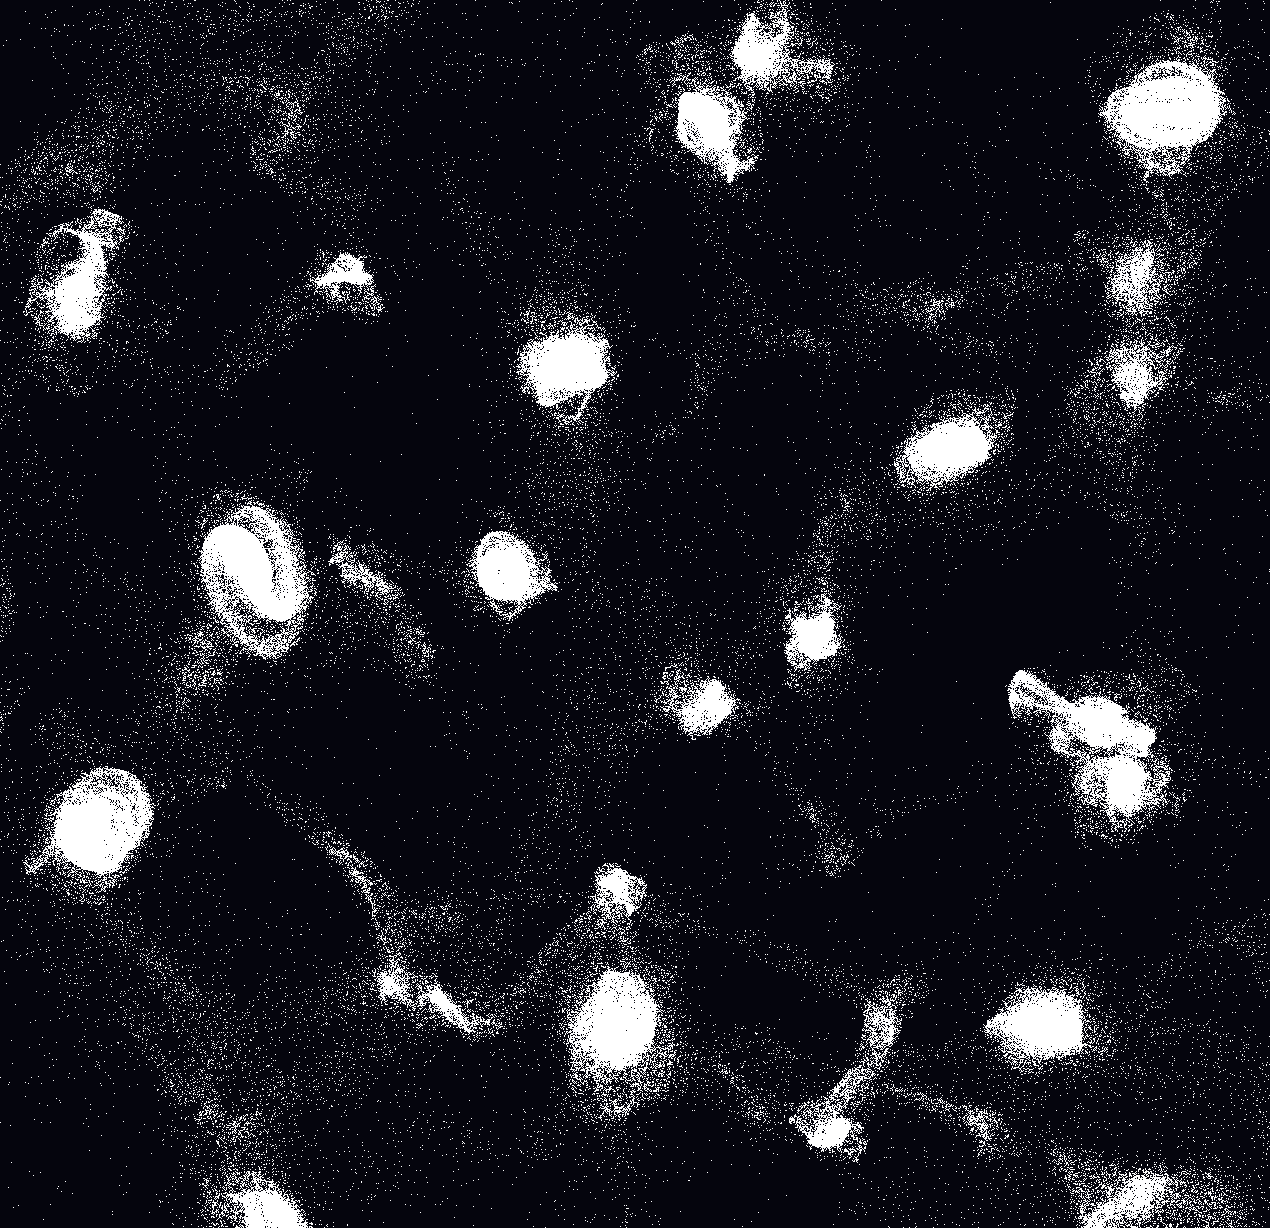
\includegraphics[width=1.0\linewidth]{images/barred_spiral} 
	\caption{Emergent barred spiral galaxy resolved using an ensemble of $N=120$ grids at a base resolution of $16^3$. The preservation of thin trailing arms and a distinct central bar proves sub-voxel force consistency.}
	\label{fig:barred_spiral}
\end{figure}

The data reveals a critical insight: finer grids ($G=64$) without an ensemble produce higher variance...
	
	\section{Discussion}
	MOG shifts the computational bottleneck from memory bandwidth to arithmetic throughput. By performing $N$ low-resolution FFTs, we leverage the massive parallel processing power of modern GPUs to recover physical isotropy. This method is particularly suited for resolving shell and ring morphologies in galactic dynamics, where sub-grid force consistency is paramount.
	
	\section{Conclusion}
	The Mixture of Grids algorithm provides a scaling advantage that allows for high-fidelity gravitational simulations on consumer-grade hardware. Future work will explore Quasi-Monte Carlo sequences (Sobol) to improve the convergence rate from $1/\sqrt{N}$ to $1/N$.
	
\end{document}